\documentclass[11pt]{article}

\usepackage[margin=1in]{geometry}
\usepackage[T1]{fontenc}
\usepackage[utf8]{inputenc}
\usepackage{lmodern}
\usepackage{booktabs}
\usepackage{array}
\usepackage{hyperref}
\usepackage{xcolor}
\usepackage{tikz}
\usetikzlibrary{arrows.meta,positioning,shapes.geometric}

\hypersetup{
  colorlinks=true,
  linkcolor=blue!50!black,
  urlcolor=blue!50!black,
  citecolor=blue!50!black
}

\title{Native Reasoning Schemas as Teacher Policies for TRM-Controlled Storyworld Factories}
\author{Patrick Dugan\\Morality Lab}
\date{May 2026}

\begin{document}
\maketitle

\begin{abstract}
We study a failure mode in a MeTTa/TRM-inspired Hermes storyworld factory: a learned tiny master planner trained from sparse synthetic trajectories failed to select the right control role on fresh diagnostic rows. In an auto-research loop over two storyworlds and three recurring defect classes, the learned planner initially matched the deterministic oracle on 0 of 16 rows. After small augmentation it improved on a held-out micro-slice, but still lacked a dependable control-plane floor. We therefore introduce a native reasoning schema: a compact set of typed diagnostic-to-role rules, expressible as MeTTa-style atoms and executable as a teacher policy for TRM supervision. On the current 16-row slice, this native schema reached 16/16 planner agreement, while the learned shadow model continued to route all rows to incorrect roles. The result is not a broad learned-generalization claim. It is a systems result: for hybrid LLM/TRM/MCP skill pipelines, native symbolic routing can supply the fast first move, prevent self-certifying planner collapse, and produce clean training labels for later TRMs that learn exceptions from real repair outcomes.
\end{abstract}

\section{Introduction}

Complex agent skills often fail not because the language model cannot produce text, but because the surrounding control plane asks the model to own too many decisions at once. In the storyworld factory studied here, a local LLM is expected to generate prose, options, reactions, clues, and short rationales, while the system must also manage context budgets, MCP packet selection, schema validity, verifier errors, effect diversity, secret-route reachability, and commit/veto decisions. Treating that entire process as one autonomous model behavior produces brittle compliance theater: the model narrates intended work, overuses global context, or certifies repairs without evidence.

The practical architecture developed in this repository separates the work. The LLM is a bounded proposal engine. MCP-style packets externalize world state. Verifiers measure structural and gameplay defects. TRMs are intended to learn compact control policies over routing, repair, and commit/veto decisions. The open problem is how to initialize the master control planner that chooses which specialized role should act next.

The key observation from the latest run is that the master planner should not begin as a weak learned model. A small model trained on sparse synthetic trajectories can memorize format without acquiring the native control logic. The fix is to put a native symbolic reasoning schema underneath learning: typed diagnostic predicates route to typed repair roles by priority. TRMs can then imitate this teacher, collect real repair outcomes, and learn where the symbolic floor is too rigid.

\section{Contribution}

This note contributes four concrete artifacts:

\begin{enumerate}
  \item A native master-control schema for the storyworld conveyor, mapping explicit failure predicates and objectives to one of nine control roles.
  \item A MeTTa-style atom file that makes the schema inspectable as symbolic routing facts.
  \item An auto-research loop with selectable planners: learned model, native teacher, or hybrid policy.
  \item A local run receipt showing 16/16 planner agreement for the native schema on the current diagnostic slice, versus 0/16 agreement for the learned shadow model on the same rows.
\end{enumerate}

The paper-worthy claim is narrow but important: native symbolic reasoning is useful as a control-plane floor for TRM-infused skills. The claim is not that the current rules prove general storyworld intelligence, nor that the final TRMs have already learned the full policy.

\section{System}

The storyworld factory uses nine conceptual control roles:

\begin{center}
\begin{tabular}{ll}
\toprule
Role & Responsibility \\
\midrule
\texttt{mcp\_context\_router} & Select the smallest useful MCP packet. \\
\texttt{world\_state\_summarizer} & Compress variables, ledger state, and local continuity. \\
\texttt{llm\_prompt\_composer} & Ask the LLM for a bounded local proposal. \\
\texttt{option\_manifold\_planner} & Repair choice diversity and intended deltas. \\
\texttt{reaction\_dynamics\_mapper} & Repair reaction contrast and state-dependent outcomes. \\
\texttt{effect\_script\_synthesizer} & Repair variable updates and effect operator variety. \\
\texttt{gate\_secret\_route\_designer} & Repair secret-route reachability and foreshadowing. \\
\texttt{validator\_repair\_critic} & Repair schema, reader, and verifier-visible defects. \\
\texttt{commit\_veto\_controller} & Accept, reject, retry, or stop based on measured deltas. \\
\bottomrule
\end{tabular}
\end{center}

Figure~\ref{fig:control-plane} shows the architecture. The native schema is intentionally small: it does not replace learning, but it stops the first routing decision from being delegated to a weak planner or a self-certifying LLM.

\begin{figure}[h]
\centering
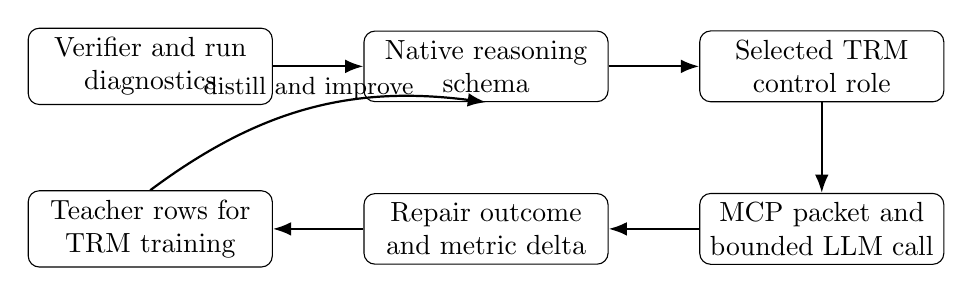
\begin{tikzpicture}[
  node distance=1.15cm,
  box/.style={draw, rounded corners, align=center, minimum width=3.1cm, minimum height=0.85cm},
  smallbox/.style={draw, rounded corners, align=center, minimum width=2.65cm, minimum height=0.75cm, font=\small},
  arrow/.style={-Latex, thick}
]
\node[box] (diag) {Verifier and run\\diagnostics};
\node[box, right=of diag] (schema) {Native reasoning\\schema};
\node[box, right=of schema] (role) {Selected TRM\\control role};
\node[box, below=of role] (mcp) {MCP packet and\\bounded LLM call};
\node[box, left=of mcp] (eval) {Repair outcome\\and metric delta};
\node[box, left=of eval] (train) {Teacher rows for\\TRM training};

\draw[arrow] (diag) -- (schema);
\draw[arrow] (schema) -- (role);
\draw[arrow] (role) -- (mcp);
\draw[arrow] (mcp) -- (eval);
\draw[arrow] (eval) -- (train);
\draw[arrow] (train.north) to[bend left=22] node[above, font=\small] {distill and improve} (schema.south);
\end{tikzpicture}
\caption{Native schema as the reasoning floor for a TRM/MCP/LLM storyworld factory. Typed diagnostics select a role before the LLM is asked for bounded creative material. Repair outcomes become supervision for later learned controllers.}
\label{fig:control-plane}
\end{figure}

\section{Native Schema}

The current schema routes failure predicates before softer objective or metric hints. The highest-priority rules are direct failure-to-role mappings:

\begin{center}
\begin{tabular}{ll}
\toprule
Predicate & Routed role \\
\midrule
\texttt{context\_overflow} & \texttt{mcp\_context\_router} \\
\texttt{insufficient\_neighbor\_context} & \texttt{mcp\_context\_router} \\
\texttt{dangling\_consequence} & \texttt{validator\_repair\_critic} \\
\texttt{unsupported\_reader\_operator} & \texttt{validator\_repair\_critic} \\
\texttt{schema\_parse\_error} & \texttt{validator\_repair\_critic} \\
\texttt{effect\_nudge\_monoculture} & \texttt{effect\_script\_synthesizer} \\
\texttt{missing\_pvalue\_refs} & \texttt{effect\_script\_synthesizer} \\
\texttt{missing\_p2value\_refs} & \texttt{effect\_script\_synthesizer} \\
\texttt{unreachable\_secret} & \texttt{gate\_secret\_route\_designer} \\
\texttt{reaction\_collapse} & \texttt{reaction\_dynamics\_mapper} \\
\texttt{option\_blandness} & \texttt{option\_manifold\_planner} \\
\texttt{too\_much\_llm\_freeform} & \texttt{llm\_prompt\_composer} \\
\texttt{no\_metric\_delta} & \texttt{commit\_veto\_controller} \\
\bottomrule
\end{tabular}
\end{center}

This policy is intentionally legible. Each row can be written as a MeTTa-style fact such as:

\begin{verbatim}
(RouteFailure context_overflow mcp_context_router)
(RouteFailure unsupported_reader_operator validator_repair_critic)
(RouteFailure effect_nudge_monoculture effect_script_synthesizer)
\end{verbatim}

The important design move is not the specific syntax. The important move is converting vague authoring defects into typed control predicates that decide the next tool, role, and training label.

\section{Experiment}

The run used the auto-research loop in the MeTTa/TRM storyworld balancer skill. It examined two storyworld artifacts:

\begin{itemize}
  \item \texttt{storyworlds/by-week/2026-W11/validated\_macbeth.json}
  \item \texttt{hermes-skills/storyworld-conveyor/working\_worlds/romeo\_sanaa\_qwen27b\_40enc/hermes\_qwen27b\_packet\_storyworld.json}
\end{itemize}

The loop ran eight iterations with post-MCP passes enabled, producing sixteen diagnostic rows. The active context budget was 8192 tokens and the recorded model tier was \texttt{9B\_Q4}. The objectives discovered in this slice were:

\begin{center}
\begin{tabular}{lr}
\toprule
Objective & Count \\
\midrule
\texttt{fit\_context\_budget} & 8 \\
\texttt{repair\_reader\_semantics} & 4 \\
\texttt{diversify\_effect\_scripts} & 4 \\
\bottomrule
\end{tabular}
\end{center}

\section{Results}

\begin{center}
\begin{tabular}{lrrl}
\toprule
Planner & Correct & Total & Notes \\
\midrule
Learned tiny planner, first auto loop & 0 & 16 & Collapsed on fresh diagnostic states. \\
Augmented learned planner & 2 & 3 & Held-out micro-slice after adding real rows. \\
Native reasoning schema & 16 & 16 & Direct diagnostic routing teacher. \\
Learned shadow model in native run & 0 & 16 & Routed to wrong role family on every row. \\
\bottomrule
\end{tabular}
\end{center}

The native run produced this role distribution, for an explicit planner agreement rate of 1.0:

\begin{center}
\begin{tabular}{lrr}
\toprule
Role & Oracle count & Native predicted count \\
\midrule
\texttt{mcp\_context\_router} & 8 & 8 \\
\texttt{validator\_repair\_critic} & 4 & 4 \\
\texttt{effect\_script\_synthesizer} & 4 & 4 \\
\bottomrule
\end{tabular}
\end{center}

By contrast, the learned shadow model assigned 12 rows to \texttt{commit\_veto\_controller} and 4 rows to \texttt{gate\_secret\_route\_designer}. Neither role was the oracle target for any row in this slice. This is the crux of the result: the learned model had a syntactically valid policy surface but no reliable native reasoning spine for the current defect classes.

\section{Interpretation}

The result looks simple because the schema is simple. That is exactly the point. In this class of agent skill, many failures are not opaque reasoning failures. They are typed, verifier-visible defects. If the whole context exceeds the budget, the next role should not be a commit/veto controller. If the reader harness rejects an operator, the next role should not be a secret-route designer. If effects have collapsed into one operator family, the next role should repair effect scripts.

This gives a stronger methodology for TRM-infused skills:

\begin{enumerate}
  \item Start with native symbolic control rules for obvious typed defects.
  \item Use those rules as a teacher policy so early TRMs learn the right action manifold.
  \item Collect real repair outcomes, including failed repairs and no-op commits.
  \item Train TRMs to learn exceptions, priorities, and context-efficiency tradeoffs.
  \item Keep the LLM as a bounded proposal source, not as the planner or judge.
\end{enumerate}

The breakthrough, if the result replicates, is not that rules beat learning. The breakthrough is that hybrid skills need a native reasoning substrate before learning can safely take over. The symbolic schema supplies the control-plane skeleton; TRMs supply compact learned adaptation; MCP supplies bounded memory; the LLM supplies local imagination.

\section{Limitations}

The present evidence is deliberately modest. The native result covers 16 rows, two storyworlds, and three objective families. The oracle is derived from the same diagnostic assumptions as the schema, so this is a proof receipt for control-plane alignment, not an independent broad benchmark. The MeTTa file is currently an inspectable symbolic representation, not a claim that the runner executes a full MeTTa interpreter. Finally, the result measures role routing, not final storyworld quality improvement.

These limits do not make the result unimportant. They define the next experiments. A useful follow-up should add more storyworlds, more defect families, human-reviewed repair outcomes, and final artifact quality deltas.

\section{Next Experiments}

The next paper-grade campaign should measure:

\begin{itemize}
  \item Held-out storyworld generalization across many source worlds and authoring styles.
  \item Defect-family coverage beyond context overflow, reader semantics, and effect-script monoculture.
  \item Native versus learned versus hybrid planner performance.
  \item Final verifier and reader-harness deltas after applying the routed repair, not only route agreement.
  \item Context efficiency: tokens retrieved, tokens generated, and avoided whole-world prompts.
  \item LLM scale sensitivity: whether 3B, 9B, and 27B proposal engines differ once the control plane owns routing and commit/veto.
\end{itemize}

\section{Conclusion}

This note documents a small but sharp systems result. A weak learned master planner failed to route real storyworld diagnostic rows. A native symbolic schema routed the same rows perfectly on the current slice and exposed the learned model's collapse mode. The likely lesson for MeTTa/TRM-infused Hermes skills is that native reasoning schemas should be treated as first-class teacher policies. They make the control plane legible, trainable, and less dependent on LLM self-management. That is a plausible path toward compact, high-capability hybrid skills in which small LLMs contribute useful proposals while symbolic and TRM layers own the hard control decisions.

\section*{Artifact References}

\begin{itemize}
  \item Native schema reference: \texttt{hermes-skills/storyworld-conveyor/skills/metta-trm-storyworld-balancer/references/native\_master\_control\_schema.md}
  \item MeTTa-style atoms: \texttt{hermes-skills/storyworld-conveyor/skills/metta-trm-storyworld-balancer/references/native\_master\_control\_schema.metta}
  \item Auto-research script: \texttt{hermes-skills/storyworld-conveyor/skills/metta-trm-storyworld-balancer/scripts/run\_master\_planner\_auto\_research\_loop.py}
  \item Native run receipt: \texttt{hermes-skills/storyworld-conveyor/trm\_corpus/master\_control\_planner\_native\_schema\_local\_001/run\_summary.json}
  \item Master planner curriculum: \texttt{hermes-skills/storyworld-conveyor/trm\_corpus/encounter\_assembly\_9trm\_seed/MASTER\_CONTROL\_PLANNER.md}
\end{itemize}

\end{document}
